\scalebox{0.8}{
    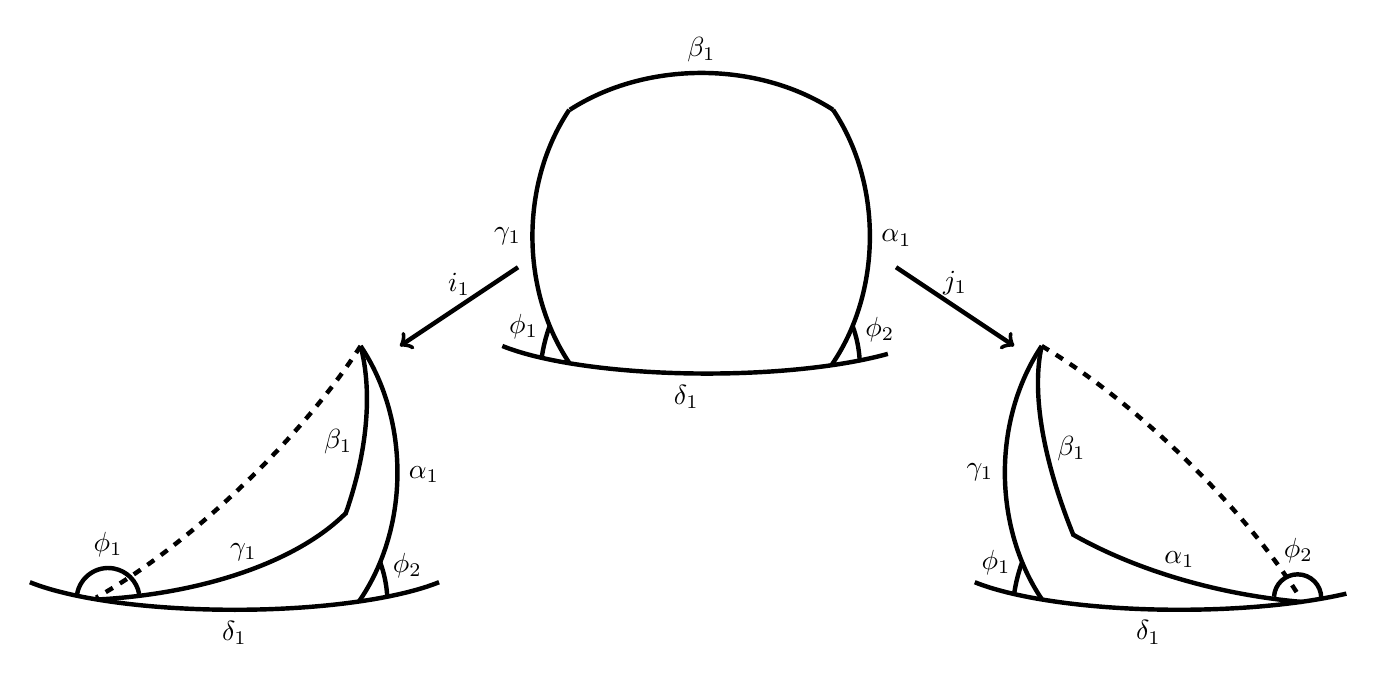
\begin{tikzpicture}
        \draw[ultra thick] (6.8, 3) arc[start angle=210, end angle = 320, x radius = 3cm, y radius = 0.7cm]  node[below, midway] {$\delta_1$};
        \draw[ultra thick] (7.65, 6) arc [start angle=140, end angle=220,x radius = 2cm, y radius = 2.5cm] node[left, midway] {$\gamma_1$};
        \draw[ultra thick] (11, 6) arc [start angle=40, end angle=-41,x radius = 2cm, y radius = 2.5cm] node[right, midway] {$\alpha_1$};
        \draw[ultra thick] (11,6) arc [start angle=50, end angle=130,x radius =2.6cm, y radius = 2cm] node[above, midway] {$\beta_1$};
        \draw[ultra thick] (7.4, 3.25) arc[start angle = 160, end angle = 172,radius=2cm] node[left, pos = 0] {$\phi_1$};
        \draw[ultra thick] (11.25, 3.25) arc[start angle = 20, end angle = 3,radius=1.5cm] node[right, pos = 0.1] {$\phi_2$};

        \draw[->, ultra thick] (7, 4) -- (5.5,3) node[above, midway] {$i_1$};
        
        \draw[ultra thick] (0.8, 0) arc[start angle=210, end angle = 330, x radius = 3cm, y radius = 0.7cm]  node[below, midway] {$\delta_1$};
        \draw[ultra thick] (1.65, -0.22) arc [start angle = -84, end angle = -26.5, x radius = 4cm, y radius = 2cm] node[above, midway] {$\gamma_1$};
        \draw[ultra thick] (5, 3) arc [start angle=40, end angle=-41,x radius = 2cm, y radius = 2.5cm] node[right, midway] {$\alpha_1$};
        \draw[ultra thick, rotate around = {-30:(5,3)}] (5,3) arc [start angle=60, end angle = 18,x radius =2cm, y radius = 3.5cm] node[left, pos=0.6] {$\beta_1$};
        \draw[ultra thick] (1.4, -0.15) arc[start angle = 170, end angle = 10,radius=0.4cm] node[above, pos = 0.5] {$\phi_1$};
        \draw[ultra thick] (5.25, 0.25) arc[start angle = 20, end angle = 3,radius=1.5cm] node[right, pos = 0.1] {$\phi_2$};
         \draw[ultra thick, dashed, rotate around = {-46:(5,3)}] (5, 3) arc[start angle=40, end angle=-43,x radius = 1cm, y radius = 3.5cm];

         \draw[->, ultra thick] (11.8, 4) -- (13.3,3) node[above, midway] {$j_1$};

        %\node [green] at (17.2, 1.8) {\textbullet};
        
        \draw[ultra thick] (12.8, 0) arc[start angle=210, end angle = 315, x radius = 3cm, y radius = 0.7cm]  node[below, midway] {$\delta_1$};
        \draw[ultra thick] (13.65, 3) arc [start angle=140, end angle=220,x radius = 2cm, y radius = 2.5cm] node[left, midway] {$\gamma_1$};
        \draw[ultra thick, rotate around = {80:(16.95, -0.25)}] (16.95, -0.25) arc [start angle=190, end angle=144.5,x radius = 2cm, y radius = 4cm] node[above, midway] {$\alpha_1$};
        \draw[ultra thick, rotate around = {-55:(13.65, 3)}] (13.65, 3) arc [start angle=200, end angle=240,x radius =5cm, y radius = 2cm] node[right, pos = 0.6] {$\beta_1$};
        \draw[ultra thick] (13.4, 0.25) arc[start angle = 160, end angle = 172,radius=2cm] node[left, pos = 0] {$\phi_1$};
        \draw[ultra thick] (17.2, -0.2) arc[start angle = 0, end angle = 177, radius=0.3cm] node[above, pos = 0.5] {$\phi_2$};
         \draw[ultra thick, dashed, rotate around = {46:(13.65, 3)}] (13.65, 3) arc[start angle=40, end angle=-42, x radius = 1cm, y radius = 3.5cm];
    \end{tikzpicture}
}